
\section{Character Building}
%todo plit into two pages and add passage for passive
\label{Section_CharacterBuilding}

\textbf{The Ancestry Tableau} - your core tool for tracking character progress.
Every Tableau is dedicated to a different species with unique modifiers and passives.
It contains the species name, places for all of the class tiles, your first passive, a place to put your life counter and a reminder text for the turn order.
To begin the game, you will choose two rank 1 classes.
The respective Class tiles are always placed in the top left in the rectangle.

\textbf{Ancestry Dice} - Whenever you get a class tile, it will cover a square on your Ancestry Tableau.
Each slot for a tile adds an Ancestry Dice.
When you cover a slot with a tile, add the printed Ancestry Dice to your dice pool.

\textbf{Level Up} - After the first and second encounter, after the event, you level up.
When you level up, you choose either a new class at rank 1, or a class you already have take one rank higher than the one you currently have. Add the new Classes Tile to your tableau, take the cards of that class, and increase your starting life by the amount stated on the new class.
You also gain a new passive. These effects are varied ways to shape your gameplay.
Most of the effects trigger at specified points during your turn. Some offer static benefits, like the one shown for the half elf which massively improves your modifier deck.

\textbf{Placement} - The class tiles have to be placed in the leftmost open slot of their rank.
Rank 1 classes go in the top row.
Rank 2 classes go in the middle row.
Rank 3 classes go in the bottom row.

\begin{figure}[ht]
	\centering
	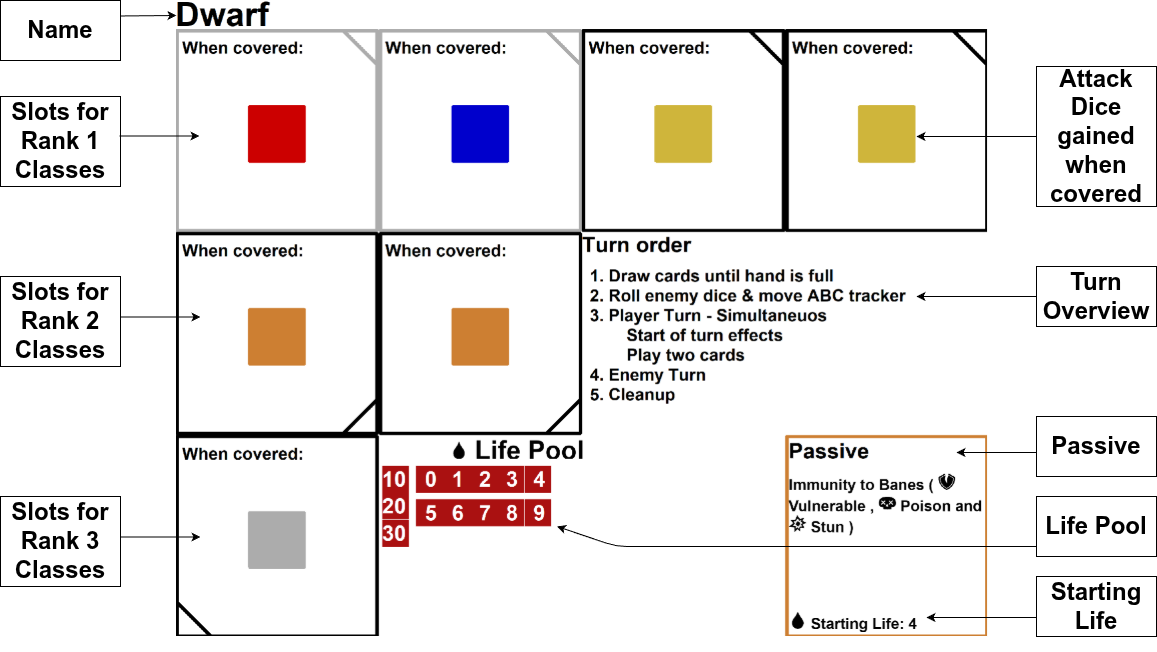
\includegraphics[width=0.9\linewidth, valign=t]{ExplanationPics/TableauRows.drawio.png}
	
\end{figure}




\begin{figure}[ht]
	\begin{minipage}[t][4.5cm][t]{0.5\textwidth}
		\textbf{Specialisation} - While every level up will grant an overall improvement to your cards, passives and modifiers, different choices will prioritize different aspects of your build.
		Rank 1 classes emphasize your modifiers, and will highlight how your species interacts with a variety of playstyles.
		Rank 2 classes have the best cards, and will allow for compressed powerful turns as you draw those cards.
		At the pinnacle stand Rank 3 classes with the best passives.
		
	\end{minipage}	
	\begin{minipage}[t][4.5cm][t]{0.5\textwidth}
		\centering
		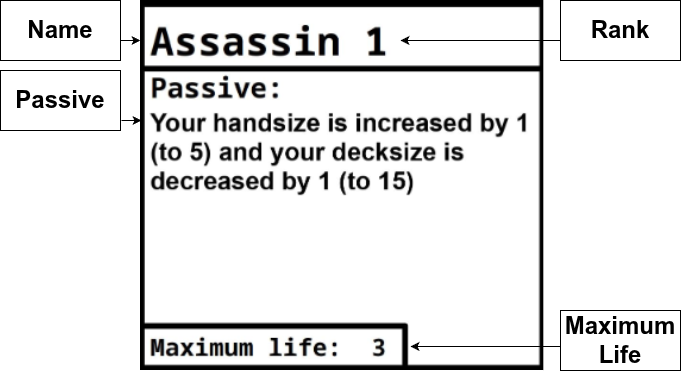
\includegraphics[width=0.9\linewidth, valign=t]{ExplanationPics/ClassShingle.drawio.png}
	\end{minipage}
\end{figure}

\begin{tcolorbox}[colframe=black, colback=white]
	Every class comes with one passive, 5 cards and around 3 life.
\end{tcolorbox}

%Tiles passgenau auf das brett zuschneiden?
%Dreiecke, Squares, Fünfecke an de seiten?
%Runde ecken etc?

